
\noindent In the path integral quantization of gauge theories, we started by guessing a quantum theory by integrating the action functional over fermion fields $\psi$, $\bar{\psi}$ and gauge boson fields $A$ to calculate transition amplitudes. \\

\noindent We noticed that there are many gauge-equivalent configurations of the gauge field that causes naive divergences, due to overcounting, in the Feynman diagram expansion. To tame this infinity, we fixed the gauge by choosing a single representative from each gauge equivalence class by inserting unity in terms of the delta functional. This introduced a nonlinear Jacobian term  $\text{det} \left( \frac{\delta G(A^\alpha)}{\delta \alpha} \right)$, where $A^\alpha$ denotes the gauge-fixed gauge field. \\

\noindent To compute this determinant, we introduced the auxiliary (classical, scalar, spinless) Grassman-valued fields $c(x)$, called Faddeev-Popov ghosts. These fields are unphysical, and must drop out during calculation. Note that the PCT-thereom does not apply to ghosts. Then transition amplitude is then defined as

\begin{equation}
\bra{\Phi_f} U \ket{\Phi_i} \equiv \int \mathcal{D} A \mathcal{D} \psi \mathcal{D} \bar{\psi} \mathcal{D} c \mathcal{D} \bar{c} \,\, e^{i S}.
\end{equation}

\noindent Where the ghosts obey the anticommutation relation as Grassman-valued fields $\{c(x), c(y)\} = 0$, and the Lagrangian density is

\begin{equation}
\mathcal{L} = -\frac{1}{4} (\partial_\mu A_\nu^a - \partial_\nu A_\mu^a)^2 + \frac{1}{2} \xi (\partial^\mu A_\mu^a)^2 + \bar{\psi} (i \slashed{\partial} - m) \psi + \bar{c}^a (-\partial^\mu \partial_\mu ) c^a + \mathcal{L}_{int} (g) .
\end{equation}

\noindent Note that the interacting bits, including the bits from the covariant derivative $D_\mu$ are absorbed into $\mathcal{L}_{int} (g)$, and everything else in the expression above is the free theory with partial derivatives $\partial_\mu$. \\

\noindent We now push forward under the belief that the perturbatively defined theory above is representative of a quantum theory, and expand in powers of the interaction term $g$ to define processes and Feynman rules of the \textbf{Yang-Mills theory}.

\subsection*{Propagators (free theory, $g=0$ part)}

\noindent The fermion propagator contributes 

\begin{equation}
\langle \bar{\psi}_{j \alpha} (x) \hat{\bar{\psi}}_{l \beta} (y) \rangle = \int \frac{d^4 k}{(2 \pi)^4} \, \left( \frac{i}{\slashed{k} - m} \right)_{\alpha \beta} \delta_{jl} e^{-i k \cdot (x-y)}.
\end{equation}

\noindent The gauge boson propagator contributes 

\begin{equation}
\langle \hat{A}_\mu^a (x) \hat{A}_\nu^b (y) \rangle = \int \frac{d^4 k}{(2 \pi)^4} \,\, \left( \eta_{\mu\nu} - (1-\xi) \frac{k_\mu k_\nu}{k^2} \right) \delta_{ab} \frac{e^{-i k \cdot (x-y)}}{k^2 + i \epsilon}.
\end{equation}

\noindent The ghost propagator contributes 

\begin{equation}
\langle \hat{c}^a (x) \hat{\bar{c}}^b (y) \rangle = \int \frac{d^4 k}{(2 \pi)^4} \,\, \frac{i}{k^2} \delta_{ab} e^{-i k \cdot (x-y)}.
\end{equation}

\noindent Recall that $a$, $b = 1,2,3$ and $\mu$, $\nu = 0,1,2,3$.

\subsection*{Vertices (interacting theory, $g \ne 0$ part)}

\noindent The interaction of two fermions and one gauge boson contributes

\begin{equation}
i g \gamma^\mu \frac{\sigma^a}{2}.
\end{equation}

\noindent The interaction of three gauge bosons contributes

\begin{equation}
g f^{abc} \left( \eta^{\mu\nu}(k-p)^\rho + \eta^{\mu\rho} (p-q)^\mu + \eta^{\rho\mu} (q-k)^\nu \right).
\end{equation}

\noindent The interaction of four gauge bosons contributes

\begin{equation}
-ig ( f^{abc} f^{cde} (\eta^{\mu\rho} \eta^{\nu\sigma} - \eta^{\mu\sigma} \eta^{\nu\rho}) + f^{ace} f^{bde} (\eta^{\mu\nu} \eta^{\rho\sigma} - \eta^{\mu\sigma} \eta^{\nu\rho}) + f^{ade} f^{bce} (\eta^{\mu\nu} \eta^{\rho\sigma} - \eta^{\mu\rho} \eta^{\nu\sigma}) ).
\end{equation}

\noindent The interaction of one gauge boson with two ghosts contributes

\begin{equation}
g f^{abc} p^\mu.
\end{equation}

\noindent (\textbf{Exercise}) And the rest of the Feynman rules for Yang-Mills theory: symmetry factors, signs, and conservations laws.  \\

\subsubsection*{Big Question 1}

\noindent Can we interpret this as a quantum theory? In other words, does this theory implicitly define the Hermitian operators $\hat{A}^\alpha$, $\hat{\psi}$, and $\hat{c}$? \\

\noindent \textbf{Yes}, it is a quantum theory, subject to a cutoff. \\

\noindent In more detail, what are the possible modes of failure for the theory to not be a valid quantum theory? \\

\noindent The first mode of failure that can occur is the time evolution operator not being unitary, or time translation not being a unitary process. To confirm that time translation in this theory is a unitary process, check that the correlation function is symmetric under the group of Poincar\'e transformation (\textbf{Exercise}). This also implies that probability is conserved. \\

\noindent The second mode of failure occurs if, after building the Fock space, we get negative norm states, such that the inner product of the system eigenstates is less than zero $\braket{\Psi | \Psi} < 0$. If this happens, then the Hamiltonian is not positive definite and we do not have a proper Hilbert space. \\

\noindent Note that there is a type of exception to this rule, which is a topic of \textit{current research}. Negative states may be able to be modded out by their subspaces to produce an effective quantum theory from the remaining subspaces with positive inner products. These remaining states are the physical, operationally defined states, and they form a convex cone from an operator algebra. The inner product in this state subspace forms a ``Hilbert subspace'', where $\braket{\Psi_{\text{phys}} | \Psi_{\text{phys}}} > 0$. \\

\subsubsection*{Big Question 2}

\noindent Is this theory, as a quantum theory, renormalizable? \\

\noindent \textbf{Yes}, thanks to the work of t'Hooft and Veltman in the REGULARIZATION AND RENORMALIZATION OF GAUGE FIELDS. They found a smart cutoff to impose that renders infinite integrals finite and retains Lorentz and gauge invariance through the technique called \textit{dimensional regularization}.\\

\noindent Note that different cutoffs can reveal different hypotheses about reality, and it is generally believed that physics is Lorentz and Poincar\'e invariant. So, a good cutoff should retain these invariances while also taming infinities of the Feynman diagram integral contributions. \\

\subsubsection*{Dimensional Regularization: An Example}

\textit{Peskin and Schroeder}, page 249. \\

\noindent In $\phi^4$ theory, as well as others, we encounter loop integrals that diverge because we are imposing too strong of a hypothesis on how the degrees of freedom of the theory behave. For example take the following loop integral that shows up in the Feynman expansion

\begin{equation}
I_n(m) = \int \frac{d^d k}{(2\pi)^d} \,\, \frac{1}{(k^2 - m^2 + i \epsilon)^n}
\end{equation}

\noindent Where $n \in \mathbb{Z}$ is the number of undetermined momenta. This produces a naive divergence of the form $\Lambda^d / \Lambda^{2n}$. \\

\noindent Note that in lower dimensions, these divergences are easier to handle. For example, if $d=2$, then $n=1$ tames the infinity. If $d=3$, $n$ must be greater than one to tame infinities of the cutoff in just three dimensions. In four dimensions, such as our usual spacetime, $n \ge 2$ is required to make the proper cancellations (e.g., need more undetermined momenta). \\

\noindent Now to evaluate that integral, we separately write out the time component integral and note that there are two poles at $k_0 = \pm( \sqrt{k^2 + m^2} -i \epsilon)$, where $k$ is just the spatial components of the $k$-vector (e.g., three spatial components of spacetime), and the $i\epsilon$ is Taylor expanded out of the square root,

\begin{equation}
I_n (m) = \int \frac{d^{d-1} k}{(2 \pi)^d} \left( \int_{-\infty}^\infty dk_0 \, \frac{1}{(k_0^2 - k^2 - m^2 + i \epsilon)^n} \right).
\end{equation}

\noindent Now, rotate the contour from running along the real axis $\Re (k_0)$ to the imaginary axis $\Im (k_0)$, effectively changing variables $k_0 \rightarrow i k_0$. Avoiding the poles, everything in the region is analytic, meromorphic and we can do this rotation.  \\

\begin{figure}[H]
	\centering
	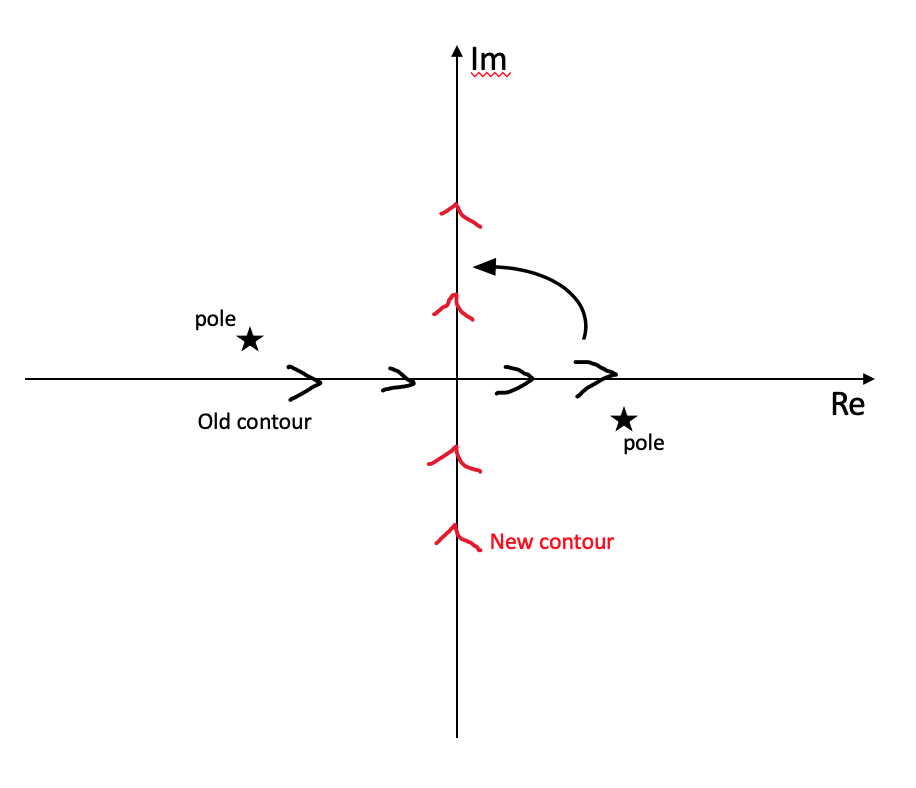
\includegraphics[width=3in]{images/contour.png}
	\caption*{Contour rotation from real-axis of $k_0$ to the imaginary axis of $k_0$.}
\end{figure}

\noindent Our integral is now

\begin{equation}
I_n(m) = -i \int \frac{d^{d-1} k}{(2 \pi)^d} \int^\infty_{-\infty} dk_0 \, \frac{1}{(k_0^2  + \omega^2)^n}.
\end{equation}

\noindent Where $\omega^2 = k^2 + m^2$. Reabsorb the time-component integral into the rest of the integrals, which we can interpret as $d$ Euclidean integrals, with the Euclidean metric, that will now exhibit spherical symmetry. Enter spherical polar coordinates

\begin{align}
I_n(m) &= -i \int_{\text{Euclidean}} \frac{d^d k}{(2 \pi)^d} \, \frac{1}{(k^2 + m^2)^n} \\
&= -\frac{i}{(2\pi)^d} \int d\Omega_d \int^\infty_0 dr \, \frac{r^{d-1}}{(r^2 + m^2)^n} \\
I_n(m) &= -\frac{i}{(2\pi)^d} \frac{(2\pi)^{\frac{d}{2}}}{\Gamma(\frac{d}{2})} \int^\infty_0 dr \, \frac{r^{d-1}}{(r^2 + m^2)^n} .
\end{align}

\noindent Make the change of variables $x = \frac{m^2}{r^2 + m^2}$

\begin{equation}
I_n(m) = \frac{m^{d-2n}}{(2\pi)^{\frac{d}{2}} \Gamma(\frac{d}{2})} \int_0^1 dx \, x^{n-\frac{d}{2}-1} (1-x)^{\frac{d}{2}-1}.
\end{equation}

\noindent This integral is a \textit{Beta function}!

\begin{equation}
I_n(m) = \frac{m^{d-2n}}{(2\pi)^{\frac{d}{2}} \Gamma(\frac{d}{2})}  \frac{\Gamma(n-\frac{d}{2}) \Gamma(\frac{d}{2})}{\Gamma(n)} = \frac{m^{d-2n}}{(2\pi)^{\frac{d}{2}}}  \frac{\Gamma(n-\frac{d}{2})}{\Gamma(n)}
\end{equation}

\noindent The gamma function has poles at negative integers, and this has divergences at $n=0,-1,-2,\dots$. The Feynman diagram expansion gives us $n$, and we are stuck with it. \\

\noindent What if $d$ is not a integer? This is the trick of dimensional regularization, as this renders the divergences finite. \\

\noindent Let $d = 4-\epsilon$, $\epsilon >0$, and study the behavior of the integral solutions as $\epsilon \rightarrow 0$.

\noindent As an example, consider the $n-2$ case (\textbf{Exercise})

\begin{align}
I_2 (m) &= \frac{m^{-\epsilon}}{(2\pi)^{2-\frac{\epsilon}{2}}} \Gamma \left(\frac{\epsilon}{2} \right) \\
&= \frac{1-\epsilon \text{log}(m)}{4\pi^2(1-\frac{\epsilon}{2} \text{log}(2\pi))} \left(\frac{2}{\epsilon} - \gamma \right) + \mathcal{O} (\epsilon^2)
\end{align}

\noindent Where $\gamma$ is the Euler-Mascheroni constant. This diverges as $\epsilon \rightarrow 0$, as expected, with the ``bad bit'' of $\frac{2}{\epsilon}$. \\

\noindent If we compare this with an integral that we've seen before, we can seee what kind of cutoff the free parameter $\epsilon$ is. Recall the diagram where we applied the momentum cutoff $|k| < \Lambda$. So, $\frac{1}{\epsilon} \sim \Lambda$.

\begin{figure}[H]
	\centering
	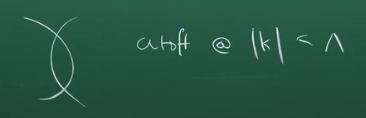
\includegraphics[width=2in]{images/firstcutoff.png}
\end{figure}
